%%%%%%%%%%%%%%%%%%%%%%%%%%%%%%%%%%%%%%%%%
% University/School Laboratory Report
% LaTeX Template
% Version 4.0 (March 21, 2022)
%
% This template originates from:
% https://www.LaTeXTemplates.com
%
% Authors:
% Vel (vel@latextemplates.com)
% Linux and Unix Users Group at Virginia Tech Wiki
%
% License:
% CC BY-NC-SA 4.0 (https://creativecommons.org/licenses/by-nc-sa/4.0/)
%
%%%%%%%%%%%%%%%%%%%%%%%%%%%%%%%%%%%%%%%%%

%----------------------------------------------------------------------------------------
%	PACKAGES AND DOCUMENT CONFIGURATIONS
%----------------------------------------------------------------------------------------

\documentclass[
	letterpaper, % Paper size, specify a4paper (A4) or letterpaper (US letter)
	10pt, % Default font size, specify 10pt, 11pt or 12pt
]{CSUniSchoolLabReport}

\addbibresource{sample.bib} % Bibliography file (located in the same folder as the template)

%----------------------------------------------------------------------------------------
%	REPORT INFORMATION
%----------------------------------------------------------------------------------------

\title{Building an Integer ALU Step 1\\ CS 3339 \\ Group: The Architects} % Report title

\author{Aaron \textsc{Reed} \& Carlo \textsc{Marroquin} \& Ryan \textsc{Bieker}} % Author name(s), add additional authors like: '\& James \textsc{Smith}'

\date{\today} % Date of the report

%----------------------------------------------------------------------------------------

\begin{document}

\maketitle % Insert the title, author and date using the information specified above

\begin{center}
	\begin{tabular}{l r}
%		Date Performed: & February 13, 2022 \\ % Date the experiment was performed
%		Partners: & Cecilia \textsc{Smith} \\ % Partner names
%		& Tajel \textsc{Khumalo} \\
		Instructor: & Professor \textsc{Klepetko} % Instructor/supervisor
	\end{tabular}
\end{center}

% If you need to include an abstract, uncomment the lines below
%\begin{abstract}
%	Abstract text
%\end{abstract}

%----------------------------------------------------------------------------------------
%	OBJECTIVE
%----------------------------------------------------------------------------------------

\section{Objective}

To introduce the process and methodology of designing a new computer circuit from scratch by coding 1-bit circuits for NAND, NOT, NOR, and 4-bit Shift.


% If you have more than one objective, uncomment the below:
%\begin{description}
%	\item[First Objective] \hfill \\
%	Objective 1 text
%	\item[Second Objective] \hfill \\
%	Objective 2 text
%\end{description}

%\subsection{Definitions}\label{definitions} % Labels provide a point for referencing, in this case with \ref{definitions} to refer to this subsection number

%\begin{description}
%	\item[Stoichiometry] The relationship between the relative quantities of substances taking part in a reaction or forming a compound, typically a ratio of whole integers.
%	\item[Atomic mass] The mass of an atom of a chemical element expressed in atomic mass units. It is approximately equivalent to the number of protons and neutrons in the atom (the mass number) or to the average number allowing for the relative abundances of different isotopes. 
%\end{description} 
 
%----------------------------------------------------------------------------------------
%	EXPERIMENTAL DATA
%----------------------------------------------------------------------------------------

\section{NAND Gate}
The NAND gate is a NOT AND operation. We took two 1-bit inputs to preform an AND operation before doing the logical NOT operation. Our 1-bit inputs were x and y.

%\begin{tabular}{l l}
	%The NAND gate is NOT and. So we took two 1-bit integers to preform an and operation before doing the logical NOT operation. %& \SI{7.28}{\gram}\\ % Scientific/technical units are output using the \SI command, see the siunitx package documentation for more information on how to use this command
	%Mass of crucible and magnesium before heating & \SI{8.59}{\gram}\\
	%Mass of crucible and magnesium oxide after heating & \SI{9.46}{\gram}\\
	%Balance used & \#4\\
	%Magnesium from sample bottle & \#1
%\end{tabular}
\begin{figure}[H] % [H] forces the figure to be placed exactly where it appears in the text
	%\centering % Horizontally center the figure
	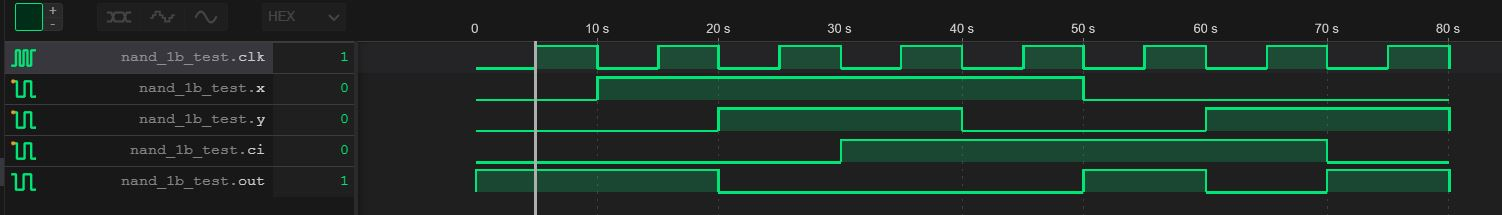
\includegraphics[width=1.2\textwidth]{nand_1b} % Include the figure
	\caption{Our NAND gate.}
\end{figure}
%----------------------------------------------------------------------------------------
%	SAMPLE CALCULATION
%----------------------------------------------------------------------------------------

\section{NOT Gate}
The NOT gate took a 1-bit input x and performed a logical NOT operation. 

\begin{figure}[H] % [H] forces the figure to be placed exactly where it appears in the text
	%\centering % Horizontally center the figure
	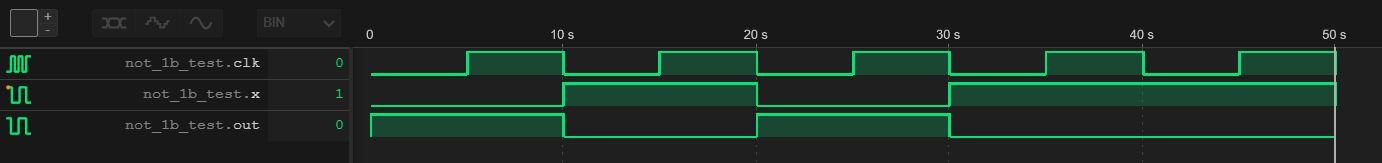
\includegraphics[width=1.2\textwidth]{not_1b} % Include the figure
	\caption{Our NOT gate.}
\end{figure}

%----------------------------------------------------------------------------------------
%	RESULTS AND CONCLUSIONS
%----------------------------------------------------------------------------------------

\section{NOR Gate}
The NOR gate took our two 1-bit inputs and preformed a logical NOT OR operation. Our inputs are x and y.

\begin{figure}[H] % [H] forces the figure to be placed exactly where it appears in the text
	%\centering % Horizontally center the figure
	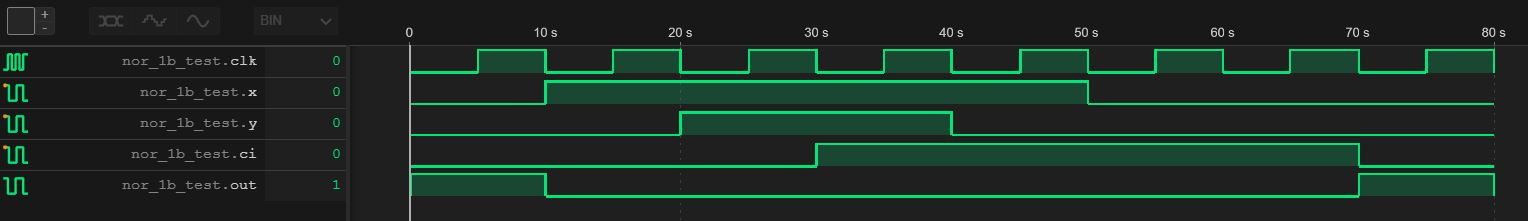
\includegraphics[width=1.2\textwidth]{nor_1b} % Include the figure
	\caption{Our NOR gate.}
\end{figure}

%----------------------------------------------------------------------------------------
%	DISCUSSION
%----------------------------------------------------------------------------------------

\section{Shift}
The shift took a 4-bit input as opposed to a 1-bit input, then one operation demonstrates the bits 1000 shifting right, and the bits 0001 shifting left.

\begin{figure}[H] % [H] forces the figure to be placed exactly where it appears in the text
	%\centering % Horizontally center the figure
	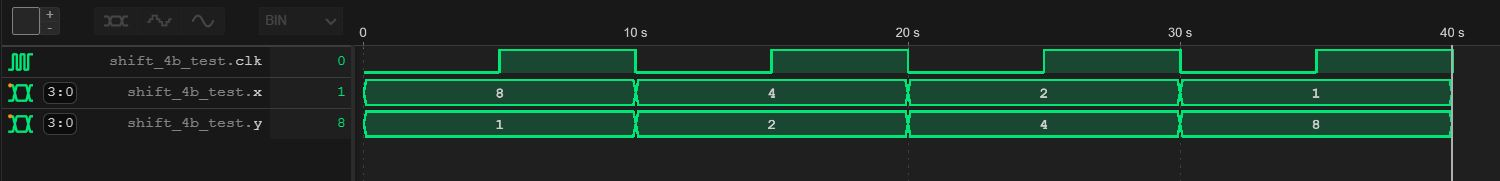
\includegraphics[width=1.2\textwidth]{shift_4b} % Include the figure
	\caption{Our 4-bit Shift.}
\end{figure}

%----------------------------------------------------------------------------------------
%	ANSWERS TO DEFINITIONS
%----------------------------------------------------------------------------------------

%\section{Answers to Definitions}

%\begin{enumerate}
%	\item The \textit{atomic weight of an element} is the relative weight of one of its atoms compared to C-12 with a weight of 12.0000000$\ldots$, hydrogen with a weight of 1.008, to oxygen with a weight of 16.00. Atomic weight is also the average weight of all the atoms of that element as they occur in nature.
%	\item The \textit{units of atomic weight} are two-fold, with an identical numerical value. They are g/mole of atoms (or just g/mol) or amu/atom.
%	\item \textit{Percentage discrepancy} between an accepted (literature) value and an experimental value is:
%		\begin{equation*}
%			\frac{\mathrm{experimental\;result} - \mathrm{accepted\;result}}{\mathrm{accepted\;result}}
%		\end{equation*}
%\end{enumerate}

%----------------------------------------------------------------------------------------
%	BIBLIOGRAPHY
%----------------------------------------------------------------------------------------
\section{Conclusion}
The shift took the longest time out of all the operations we had to code. We also struggled getting on the same page in terms of what coding software we were using, especially since we all have varying experience with Verilog and Latex, but once we got on the same page we all seemed to work well together.

%\printbibliography % Output the bibliography

%----------------------------------------------------------------------------------------

\end{document}
